\section{Introduction}
MaskGIT 是一個 Generative Image Transformer,它使用 Transformer 架構來生成與修復圖片。

利用雙向 Transformer 來同時預測所有 token,從而提升生成速度


這次的作業是要實作 Multi-head Attention 來嘗試圖片修補的任務,判斷分數的標準是使用 FID score(越小越好),目標要低於 40,並且還要說明訓練的設定與策略。



This is an introduction section. \cite{chang2022maskgit}

\begin{figure}[htbp]
    \centering
    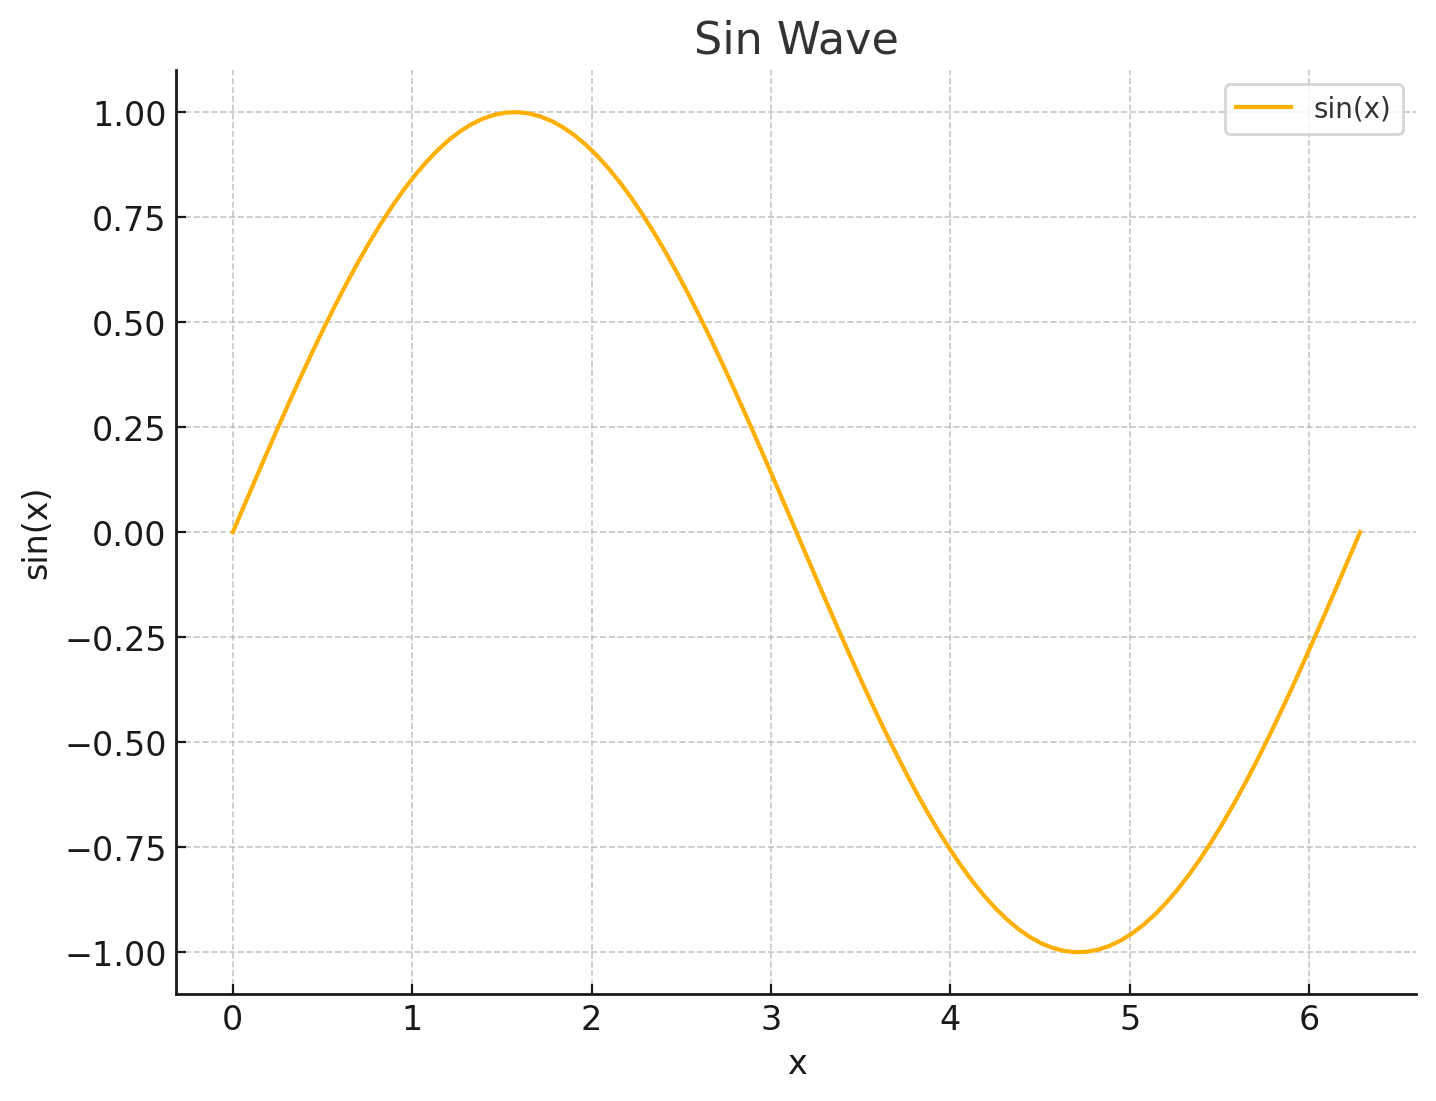
\includegraphics[width=0.8\textwidth]{figures/fig1.png}
    \caption{The architecture of MaskGIT model. The model consists of a transformer encoder and decoder, where the encoder processes the input image and the decoder generates the masked tokens. The training process involves randomly masking tokens and predicting them, while inference uses a non-autoregressive approach with iterative refinement.}
    \label{fig:maskgit_architecture}
\end{figure} 